\begin{figure}[h!] % Gunakan \begin{figure*} untuk memasukkan Gambar
	\centering
	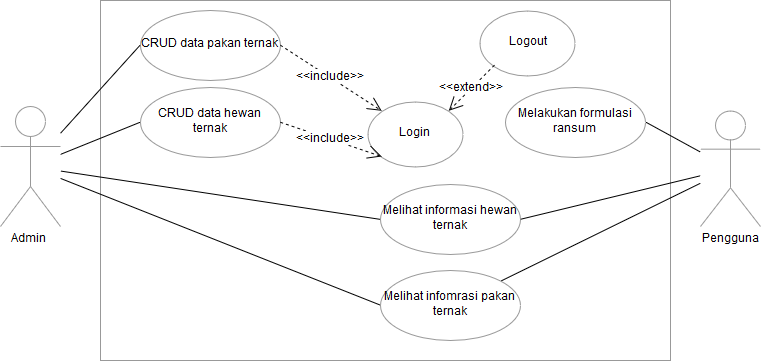
\includegraphics[width=250pt]{use_case_iterasi1.png}
	\caption{\textit{Use case} diagram sistem formulasi}
	\label{fig:usecase1}
\end{figure}

\begin{figure}[h!] % Gunakan \begin{figure*} untuk memasukkan Gambar
	\centering
	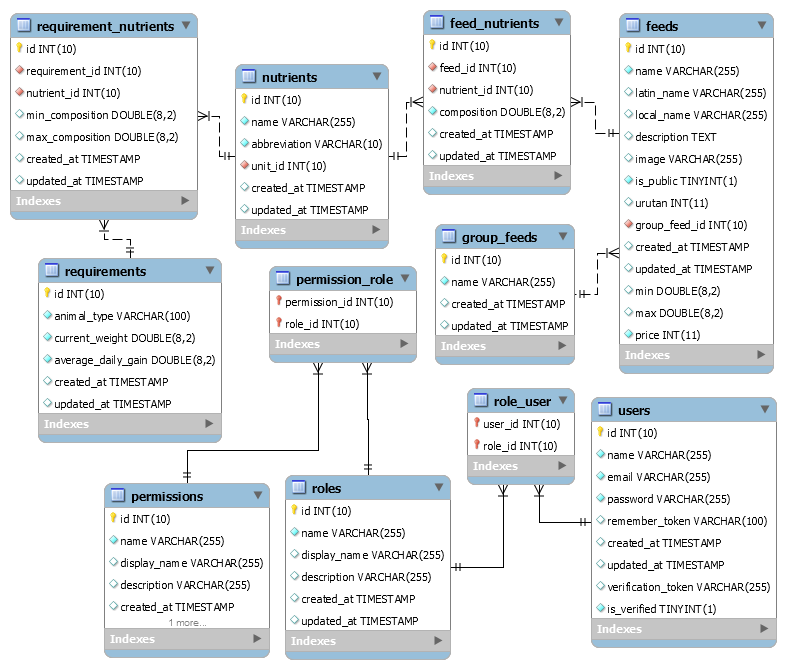
\includegraphics[width=250pt]{erd1.png}
	\caption{Diagram relasi antar tabel}
	\label{fig:erd1}
\end{figure}

\begin{figure}[h!] % Gunakan \begin{figure*} untuk memasukkan Gambar
	\centering
	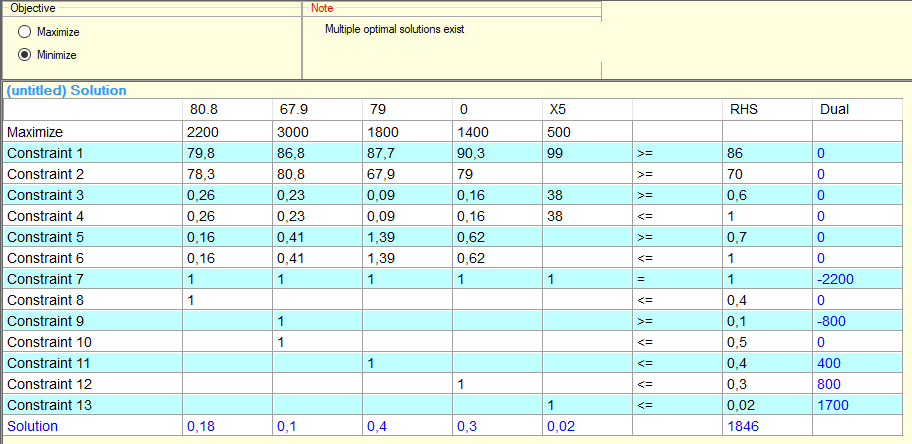
\includegraphics[width=250pt]{pom_qm1.png}
	\caption{Hasil penerapan \textit{linier programming} pada aplikasi POM QM}
	\label{fig:pomqm1}
\end{figure}

\begin{figure}[h!] % Gunakan \begin{figure*} untuk memasukkan Gambar
\centering
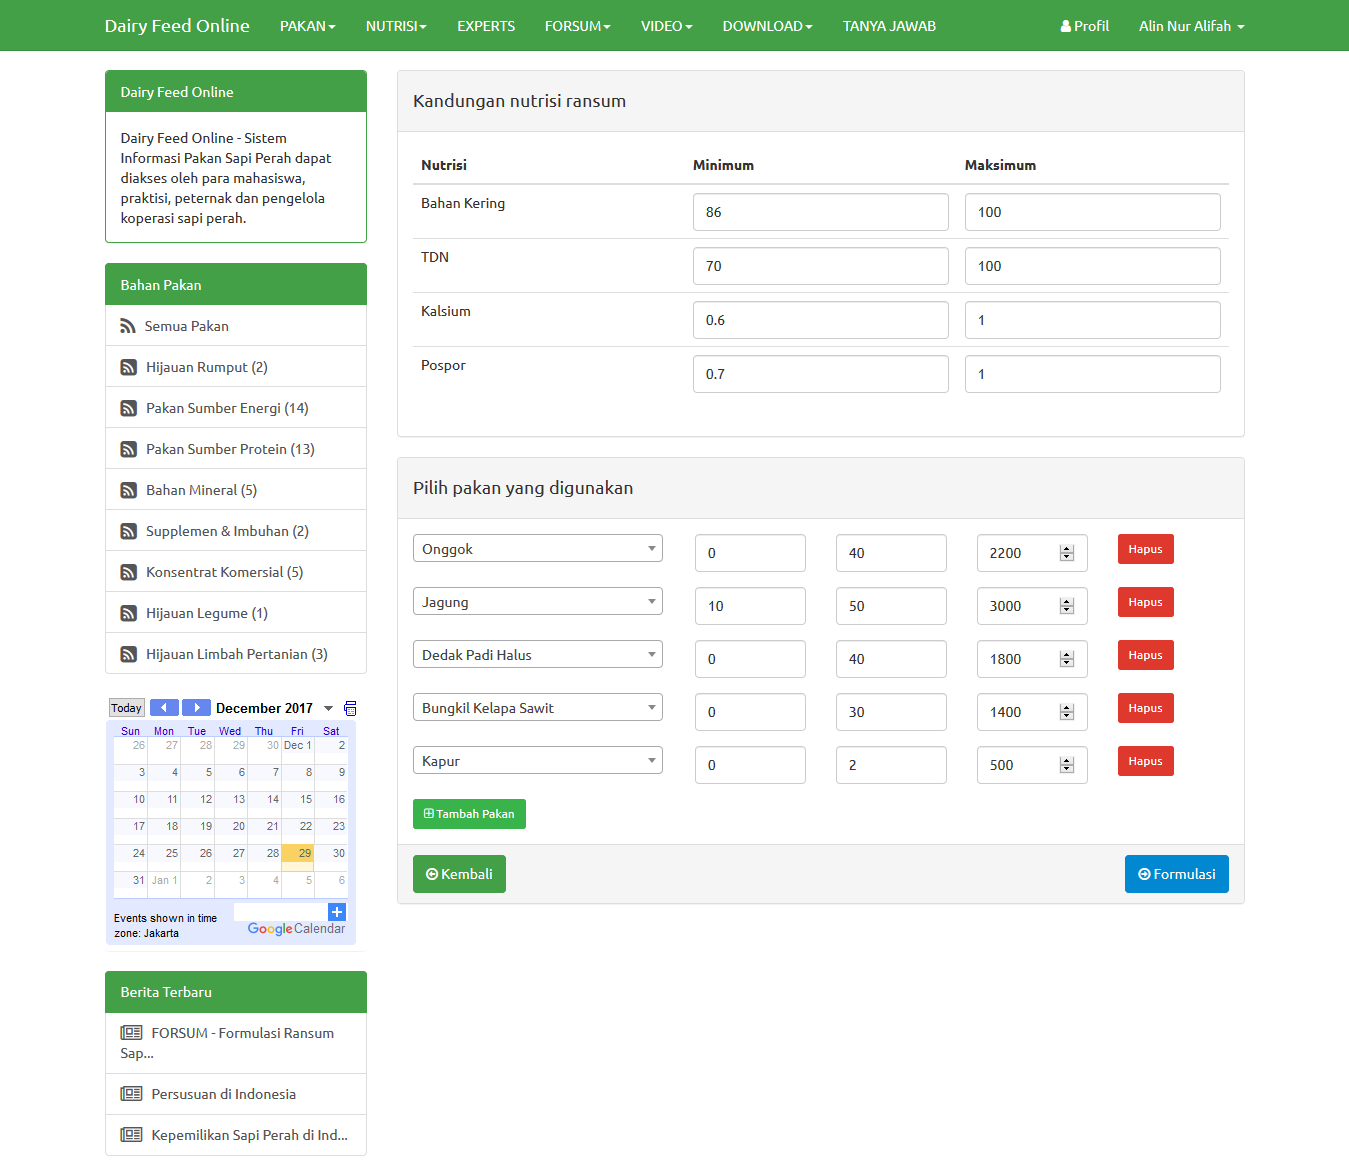
\includegraphics[width=250pt]{prototype1.png}
\caption{\textit{Prototype} halaman input formulasi}
\label{fig:pt1_1}
\end{figure}

\begin{figure}[h!] % Gunakan \begin{figure*} untuk memasukkan Gambar
\centering
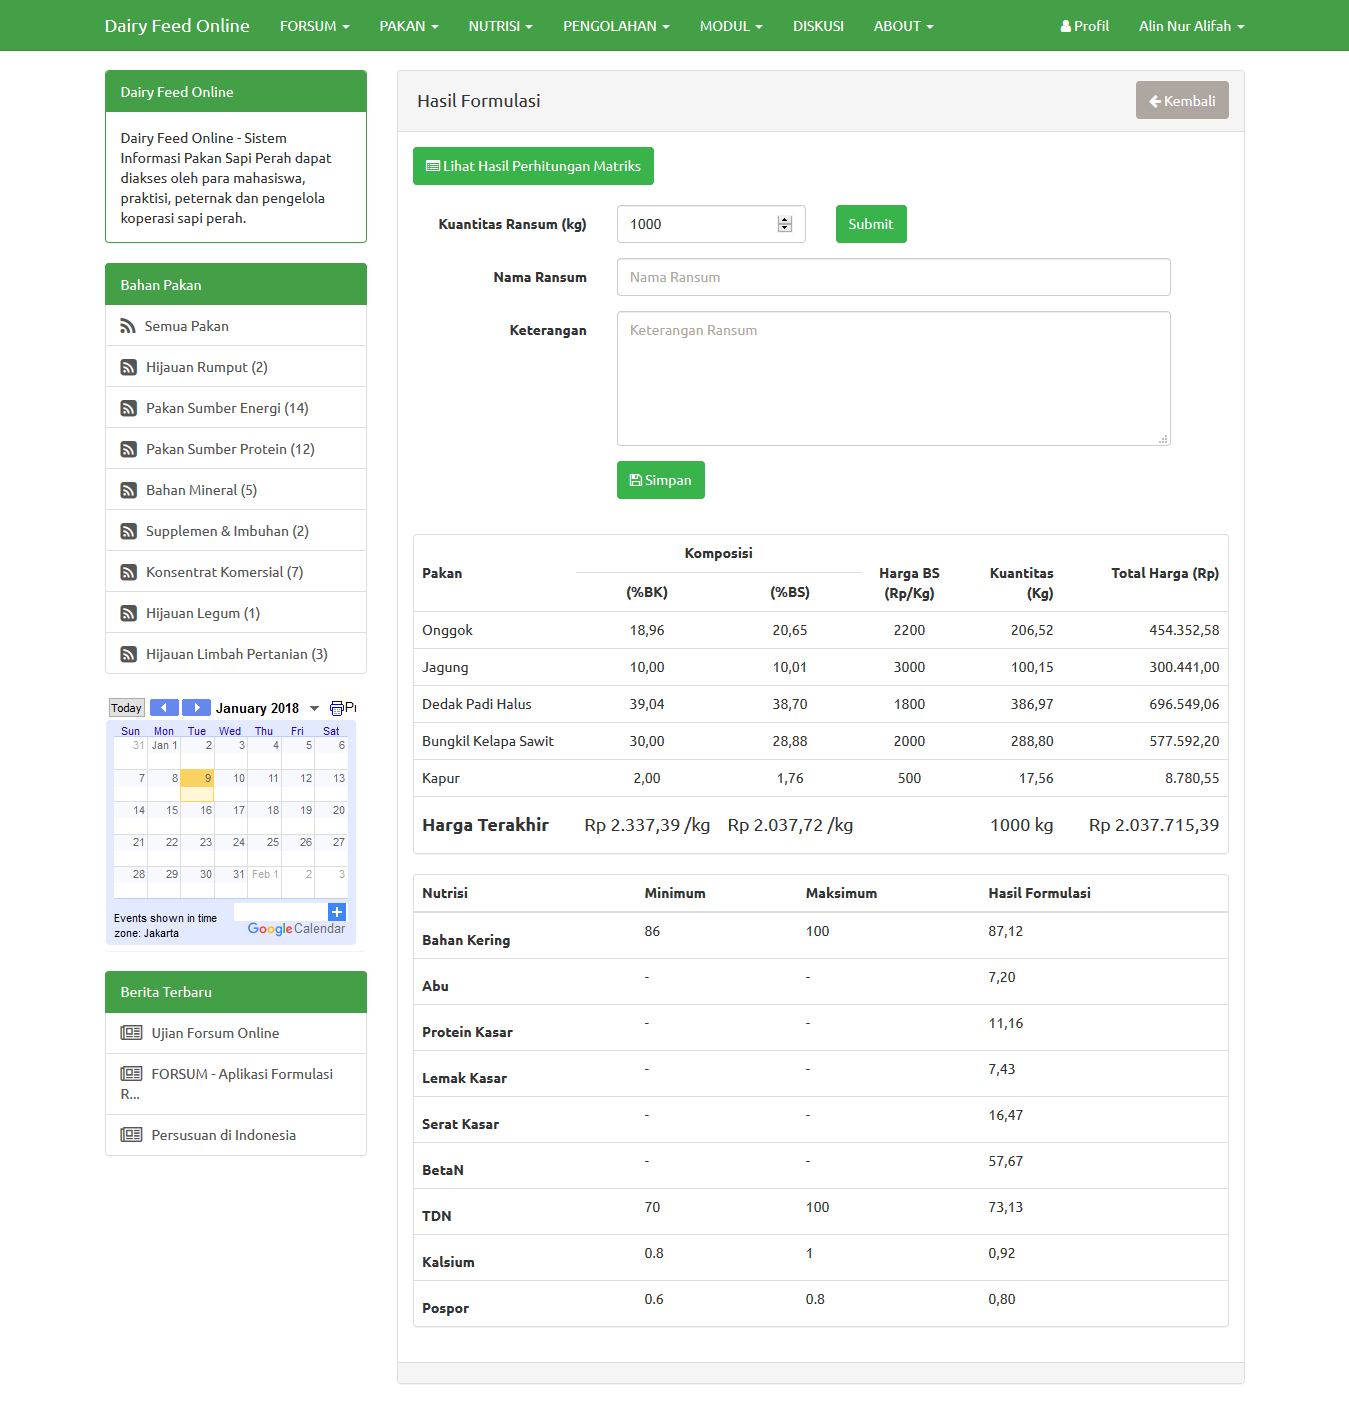
\includegraphics[width=250pt]{prototype1_2.png}
\caption{\textit{Prototype} halaman hasil formulasi}
\label{fig:pt1_2}
\end{figure}

\begin{figure}[h!] % Gunakan \begin{figure*} untuk memasukkan Gambar
	\centering
	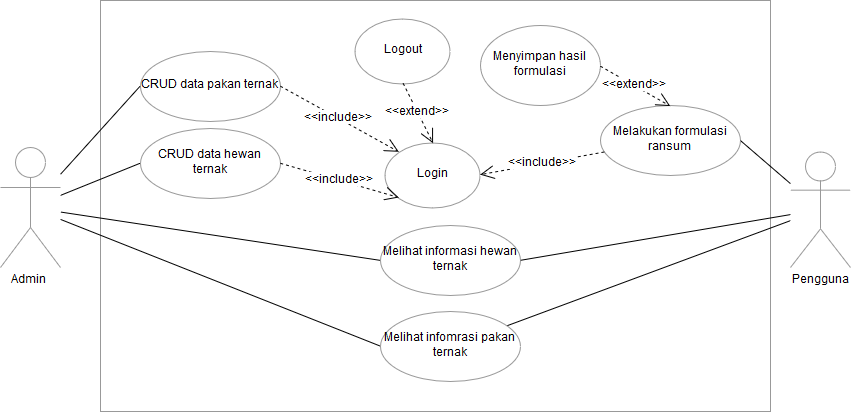
\includegraphics[width=250pt]{usecase2.png}
	\caption{\textit{Use case} diagram iterasi 2}
	\label{fig:usecase1}
\end{figure}

\begin{figure}[h!] % Gunakan \begin{figure*} untuk memasukkan Gambar
	\centering
	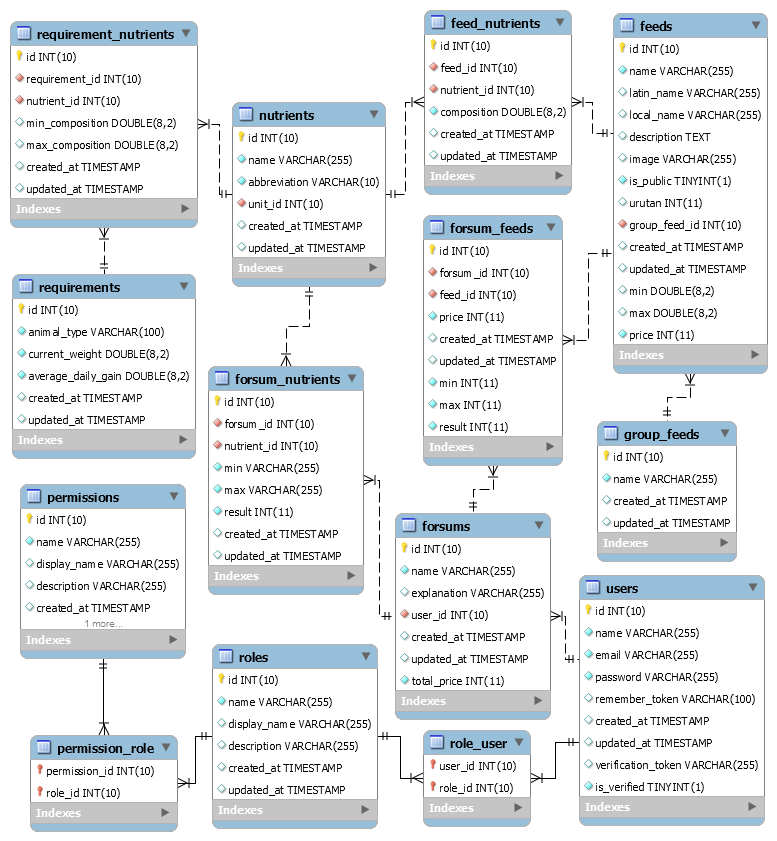
\includegraphics[width=250pt]{erd2.png}
	\caption{Diagram relasi antar tabel iterasi 2}
	\label{fig:erd1}
\end{figure}

\begin{figure}[h!] % Gunakan \begin{figure*} untuk memasukkan Gambar
	\centering
	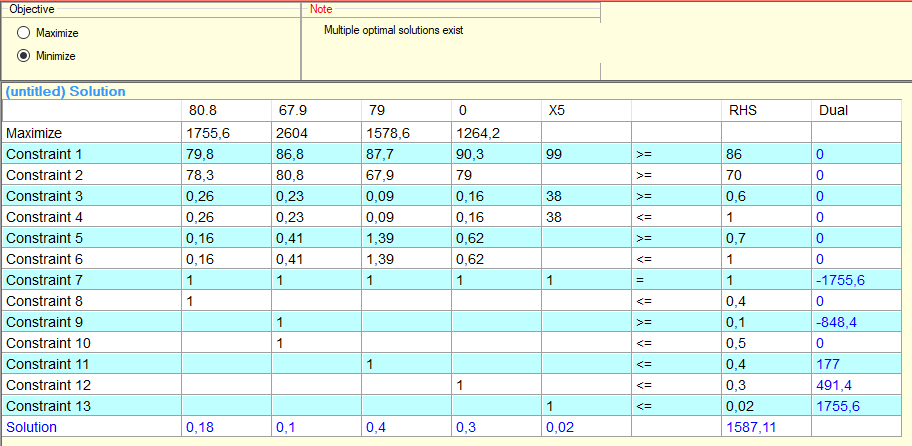
\includegraphics[width=250pt]{pom_qm2.png}
	\caption{Hasil \textit{linier programming} menggunakan aplikasi POM QM}
	\label{fig:pom_qm2}
\end{figure}

\begin{figure}[h!] % Gunakan \begin{figure*} untuk memasukkan Gambar
\centering
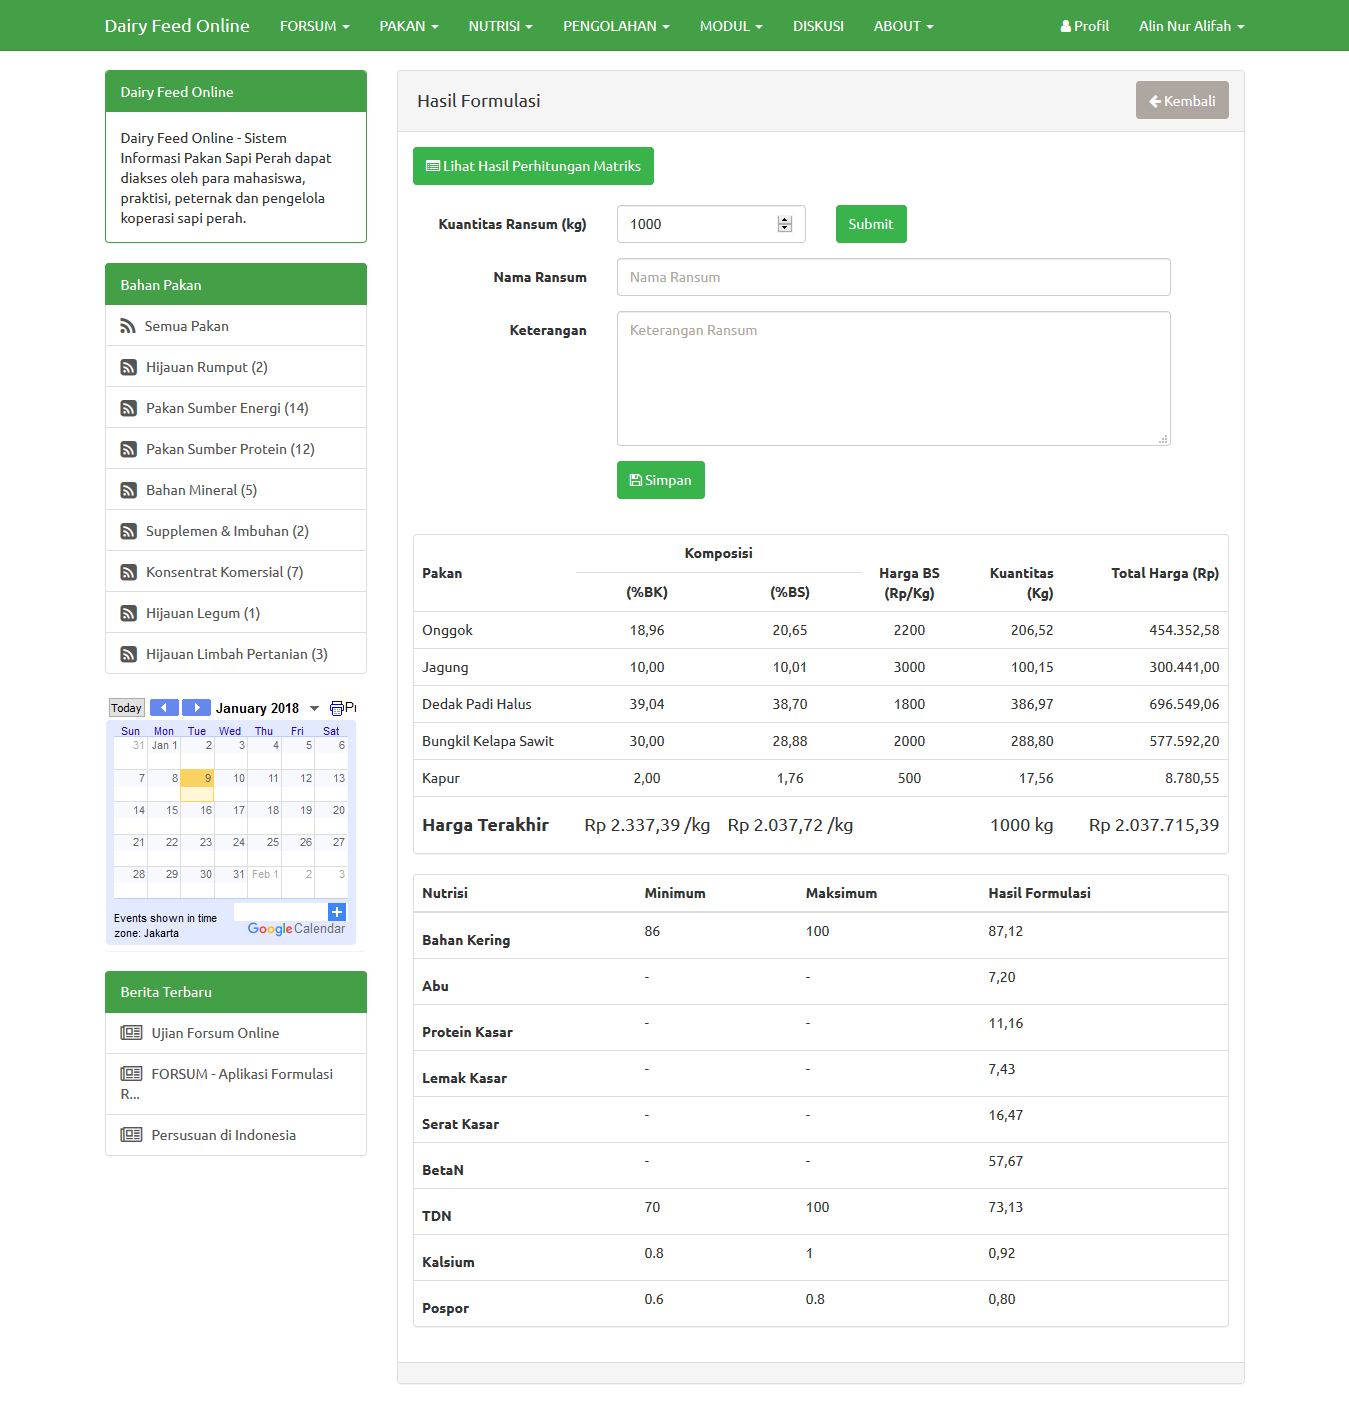
\includegraphics[width=250pt]{prototype2.png}
\caption{\textit{Prototype }hasil dengan bahan segar}
\label{fig:pt2}
\end{figure}

\begin{figure}[h!] % Gunakan \begin{figure*} untuk memasukkan Gambar
	\centering
	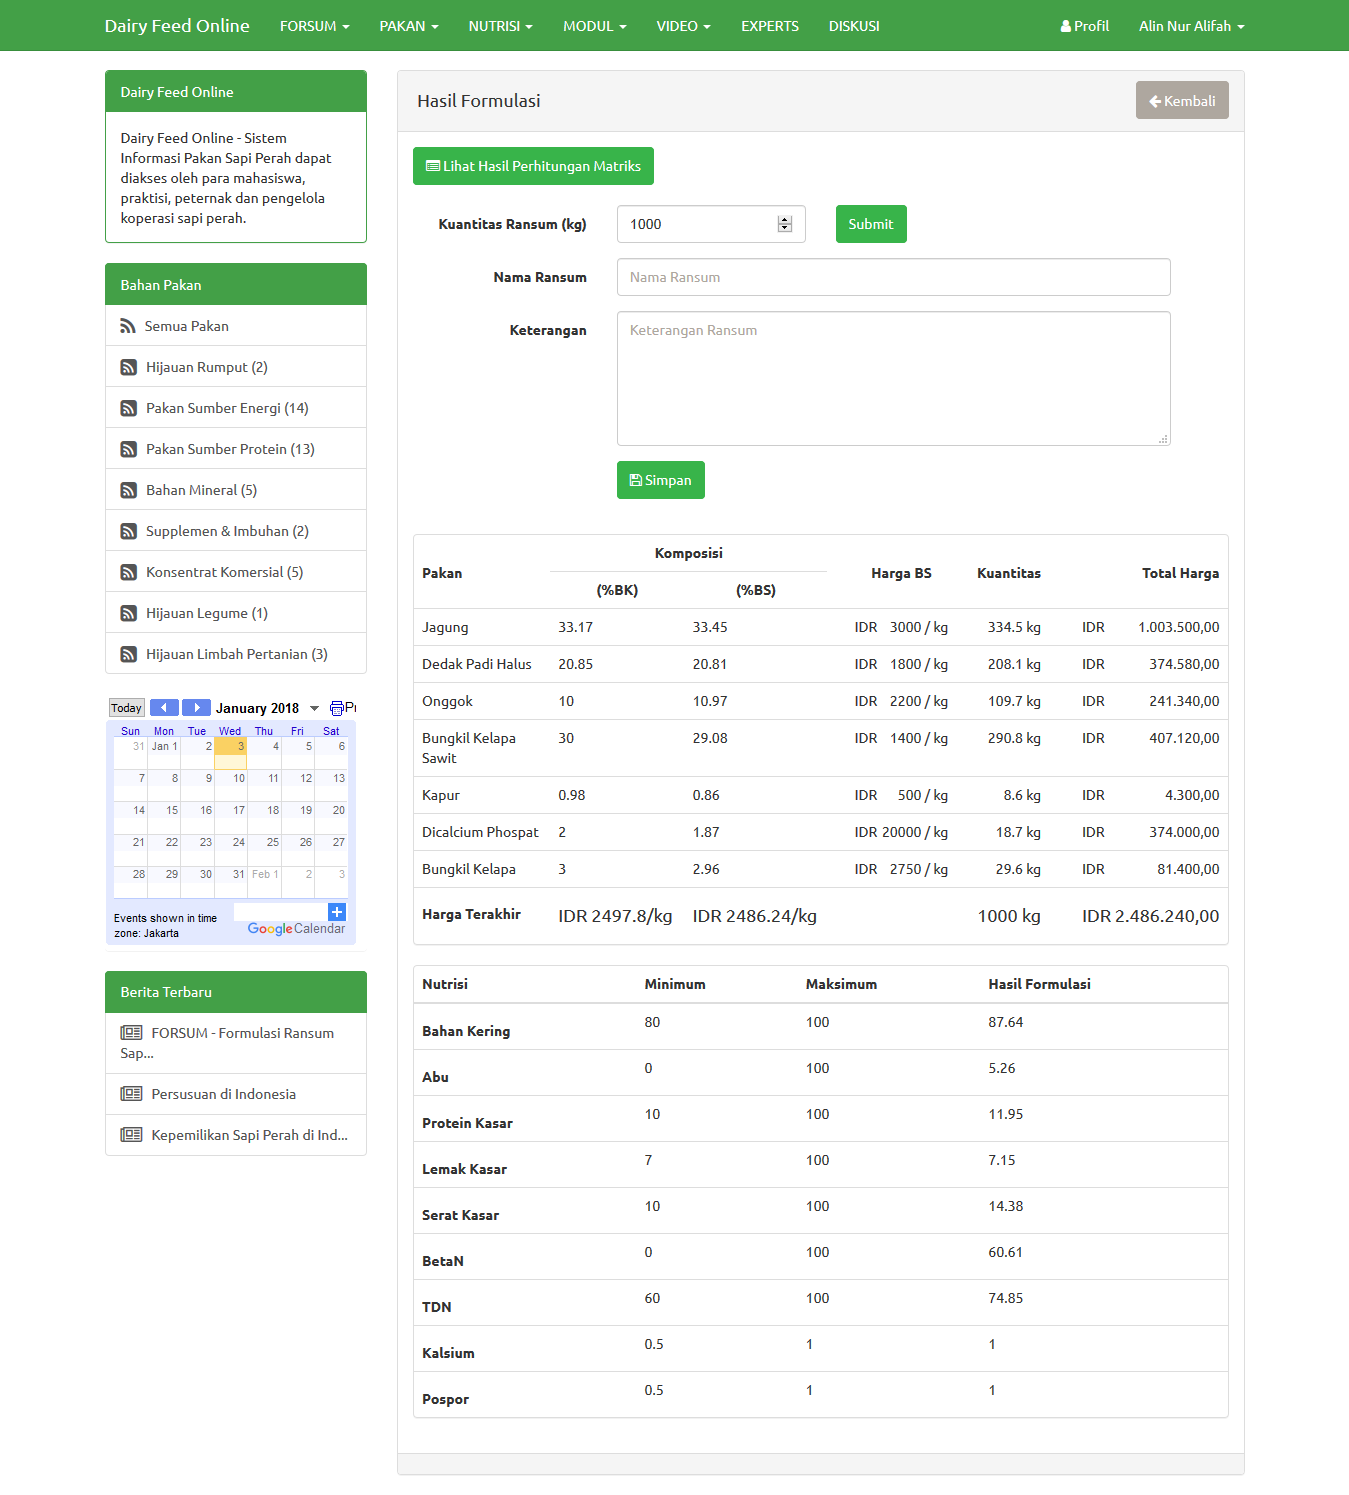
\includegraphics[width=250pt]{feedback1.png}
	\caption{Hasil formulasi ransum pada aplikasi Dairy Feed}
	\label{fig:fd1}
\end{figure}

\begin{figure}[h!] % Gunakan \begin{figure*} untuk memasukkan Gambar
	\centering
	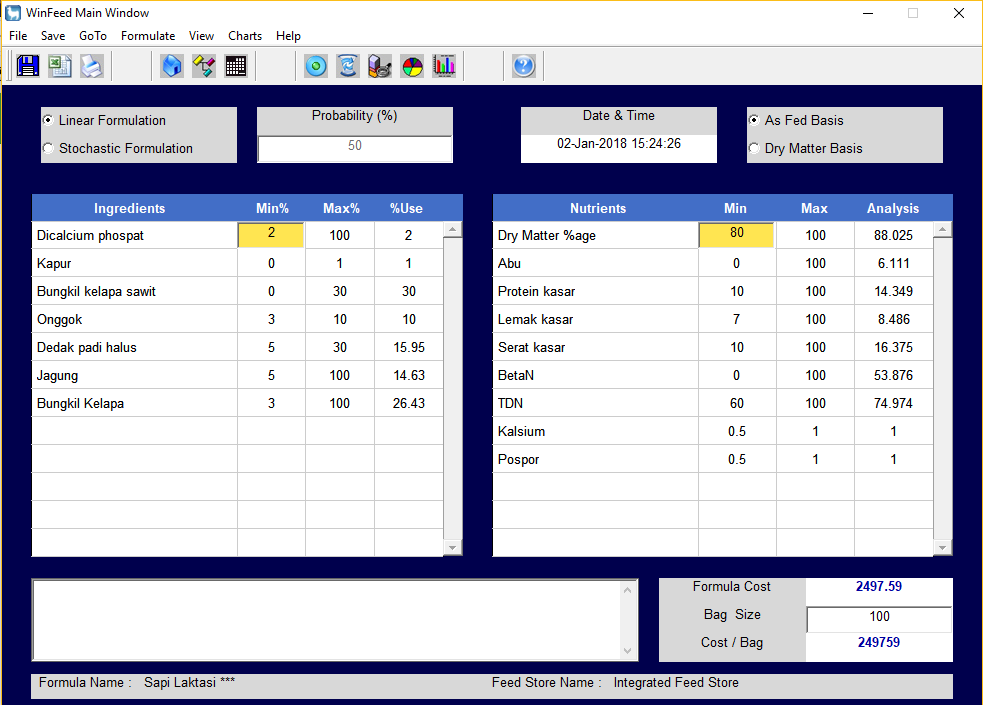
\includegraphics[width=250pt]{feedback_winfeed1.png}
	\caption{Hasil formulasi ransum menggunakan aplikasi WinFeed}
	\label{fig:fd_wf2}
\end{figure}

\begin{table}[h!]
	\centering
	\caption{Daftar Kebutuhan Pengguna}
	\label{my-label}
	\begin{tabular}{ p{2.5cm}p{5cm}  }
		\hline
		Kebutuhan & Keterangan \\ \hline
		Melakukan formulasi ransum & Pengguna dapat melakukan formulasi dengan dapat mengatur nilai nutrisi kebutuhan ternak dan jumlah pakan yang akan digunakan untuk formulasi \\
		Mengelola data pakan & Admin dapat mengelola data pakan yang bisa digunakan untuk formulasi serta kandungan nutrisi yang berada pada pakan \\
		Mengelola data ternak & Admin dapat mengelola data ternak serta kebutuhan nutrisi pada ternak \\
		Melihat informasi ternak dan kebutuhan nutrisinya & Pengguna dapat melihat informasi ternak dan kebutuhan nutrisinya \\
		Melihat informasi pakan dan kandungan nutrisinya & Pengguna dapat melihat informasi pakan dan kandungan nutrisinya \\ \hline
	\end{tabular}
\end{table}

\begin{table}[h!]
	\centering
	\caption{Bahan pakan dan batasan penggunaannya pada pengujian}
	\label{my-label}
	\begin{tabular}{p{3cm}p{1.5cm}p{0.75cm}p{0.75cm}}
		\hline
		Bahan Pakan        & Harga (Rp/kg) & Min (\%) & Max (\%) \\ \hline
		Dicalcium  phospat & 10000         & 0        & 100      \\
		Dedak padi halus   & 1500          & 10       & 30       \\
		Pollard            & 2300          & 20       & 100      \\
		Bungkil kedelai    & 7000          & 2        & 100      \\
		Onggok             & 2200          & 10       & 100      \\
		Bungkil Sawit      & 2500          & 10       & 25       \\
		Molases            & 2000          & 10       & 15       \\
		Kapur              & 750           & 0        & 2        \\
		Jagung             & 3000          & 15       & 100      \\ \hline
	\end{tabular}
\end{table}

\begin{table}[h!]
	\centering
	\caption{Batasan kebutuhan nutrien pada pengujian}
	\label{my-label}
	\begin{tabular}{p{3.5cm}p{0.75cm}p{0.75cm}}
		\hline
		Nutrien            & Min & Max \\ \hline
		Bahan kering (\%)  & 86  & 100 \\
		Abu (\%)           & 0   & 100 \\
		Protein kasar (\%) & 15  & 100 \\
		Lemak kasar (\%)   & 0   & 100 \\
		Serat kasar (\%)   & 0   & 100 \\
		BetaN (\%)         & 0   & 100 \\
		TDN                & 70  & 100 \\
		Kalsium (\%)       & 1   & 100 \\
		Phospor (\%)       & 1   & 100 \\ \hline
	\end{tabular}
\end{table}

\begin{table}[h!]
	\centering
	\caption{Hasil formulasi ransum dan komposisi bahan pakan}
	\label{my-label}
	\begin{tabular}{p{3.5cm}p{0.75cm}p{0.75cm}}
		\hline
		Hasil                   & DF    & WF    \\ \hline
		Dicalcium  phospat (\%) & 1.72  & 1.72  \\
		Dedak padi halus (\%)   & 10    & 10    \\
		Pollard (\%)            & 32.01 & 32.01 \\
		Bungkil kedelai (\%)    & 8.09  & 8.09  \\
		Onggok (\%)             & 10    & 10    \\
		Bungkil Sawit (\%)      & 11.19 & 11.19 \\
		Molases (\%)            & 10    & 10    \\
		Kapur (\%)              & 2     & 2     \\
		Jagung (\%)             & 15    & 15 	\\ \hline
	\end{tabular}
\end{table}

\begin{table}[h!]
	\centering
	\caption{Nilai nutrient pada hasil formulasi ransum}
	\label{my-label}
	\begin{tabular}{p{3.5cm}p{0.75cm}p{0.75cm}}
		\hline
		Nutrien            & DF    & WF    \\ \hline
		Bahan kering (\%)  & 86    & 86    \\
		Abu (\%)           & 5.34  & 5.34  \\
		Protein kasar (\%) & 15    & 15    \\
		Lemak kasar (\%)   & 4.33  & 4.33  \\
		Serat kasar (\%)   & 9.05  & 9.05  \\
		BetaN (\%)         & 62.61 & 62.61 \\
		TDN (\%)           & 72.45 & 72.45 \\
		Kalsium (\%)       & 1.42  & 1.42  \\
		Phospor (\%)       & 1     & 1 	   \\ \hline
	\end{tabular}
\end{table}

\begin{table}[h!]
	\centering
	\caption{Daftar Kebutuhan Pengguna}
	\label{my-label}
	\begin{tabular}{ p{2.5cm}p{5cm}  }
		\hline
		Kebutuhan                            & Keterangan                                                                                                    \\ \hline
		Menyimpan hasil formulasi            & Pengguna dapat menyimpan hasil ransum untuk dapat diakses kembali dan dicetak                                 \\
		Perhitungan hasil dengan bahan segar & Hasil yang didapatkan dari linier merupakan komposisi bahan segar                                             \\
		Registrasi                           & Pengguna wajib melakukan login sebelum melakukan formulasi dan pengguna dapat membuat akun melalui registrasi	   \\ \hline
	\end{tabular}
\end{table}

\begin{table}[h!]
	\centering
	\caption{Bahan pakan dan batasan penggunaannya pada pengujian}
	\label{my-label}
	\begin{tabular}{p{2.5cm}p{1cm}p{0.5cm}p{0.5cm}p{0.5cm}p{0.5cm}}
		\hline
		&&\multicolumn{2}{c}{Pengujian 1} & \multicolumn{2}{c}{Pengujian 2} \\ \hline
		Bahan Pakan       & Harga (Rp/kg) & Min (\%) & Max (\%) & Min (\%) & Max (\%) \\ \hline
		Jagung            & 3000          & 5        & 100      & 10       & 100      \\
		Dedak padi halus  & 1800          & 5        & 30       & 0        & 30       \\
		Onggok            & 2200          & 3        & 10       & 0        & 100      \\
		Bungkil Sawit     & 1400          & 0        & 30       & 0        & 25       \\
		Kapur             & 500           & 0        & 1        & 0        & 1        \\
		Dicalcium Phospat & 20000         & 2        & 100      & 0        & 100      \\
		Bungkil Kelapa    & 2750          & 3        & 100      & 30       & 100      \\ \hline
	\end{tabular}
\end{table}

\begin{table}[h!]
	\centering
	\caption{Batasan kebutuhan nutrien pada pengujian}
	\label{my-label}
	\begin{tabular}{p{3.5cm}p{0.5cm}p{0.5cm}p{0.5cm}p{0.5cm}}
		\hline
		&\multicolumn{2}{c}{Pengujian 1} & \multicolumn{2}{c}{Pengujian 2} \\ \hline
		Nutrien            & Min         & Max & Min & Max \\ \hline
		Bahan kering (\%)  & 80          & 100 & 0   & 100 \\
		Abu (\%)           & 0           & 100 & 0   & 100 \\
		Protein kasar (\%) & 10          & 100 & 15  & 100 \\
		Lemak kasar (\%)   & 7           & 100 & 0   & 100 \\
		Serat kasar (\%)   & 10          & 100 & 0   & 100 \\
		BetaN (\%)         & 0           & 100 & 0   & 100 \\
		TDN                & 60          & 100 & 65  & 100 \\
		Kalsium (\%)       & 0.5         & 1   & 1   & 100 \\
		Phospor (\%)       & 0.5         & 1   & 0.5 & 100 \\ \hline
	\end{tabular}
\end{table}

\begin{table}[h!]
	\centering
	\caption{Nilai komposisi pakan pada hasil formulasi}
	\label{my-label}
	\begin{tabular}{p{3.5cm}p{0.5cm}p{0.5cm}p{0.5cm}p{0.5cm}}
		\hline
		&\multicolumn{2}{c}{Pengujian 1} & \multicolumn{2}{c}{Pengujian 2} \\ \hline
		Hasil                  & DF          & WF      & DF   & WF      \\ \hline
		Jagung (\%)            & 33.17       & 14.63   & 10      & 10      \\
		Dedak padi halus (\%)  & 20.85       & 15.95   & 30      & 30      \\
		Onggok (\%)            & 10          & 10      & 2.14    & 1.9     \\
		Bungkil Sawit (\%)     & 30          & 30      & 25      & 25      \\
		Kapur (\%)             & 0.98        & 1       & 1       & 1       \\
		Dicalcium Phospat (\%) & 2           & 2       & 1.86    & 2.1     \\
		Bungkil Kelapa (\%)    & 3           & 26.43   & 30      & 30      \\
		Harga BK (Rp/kg)       & 2497      & 2497 & 2741 & 2786 \\ \hline
	\end{tabular}
\end{table}
\begin{table}[h!]
	\centering
	\caption{Nilai nutrien pada hasil formulasi}
	\label{my-label}
	\begin{tabular}{p{3.5cm}p{0.5cm}p{0.5cm}p{0.5cm}p{0.5cm}}
		\hline
		&\multicolumn{2}{c}{Pengujian 1} & \multicolumn{2}{c}{Pengujian 2} \\ \hline
		Nutrien            & DF          & WF    & DF    & WF    \\ \hline
		Bahan kering (\%)  & 87.64       & 88.03 & 88.61 & 88.53 \\
		Abu (\%)           & 5.26        & 6.11  & 7.81  & 8.89  \\
		Protein kasar (\%) & 11.95       & 14.35 & 15.31 & 17.26 \\
		Lemak kasar (\%)   & 7.15        & 8.49  & 9.27  & 10.44 \\
		Serat kasar (\%)   & 14.38       & 16.38 & 14.60 & 18.51 \\
		BetaN (\%)         & 60.61       & 53.88 & 49.7  & 56.7  \\
		TDN (\%)           & 74.85       & 74.98 & 73.3  & 83.16 \\
		Kalsium (\%)       & 1           & 1     & 1     & 1     \\
		Phospor (\%)       & 1           & 1     & 1.17  & 1.26  \\ \hline
	\end{tabular}
\end{table}